%% Digital Systems
%% Continuous System Equivalence
\def\FileDate{98/12/02}
\def\FileVersion{1.0}
% ----------------------------------------------------------------
% Notes pages *********************************************************
% ----------------------------------------------------------------

In many cases, e.g. signal processing, control systems, etc., we want to design a digital system so that it behaves
(dynamically and in steady-state) the same as a continuous
system. A digital system that has the same input-behaviour as
a (sampled) continuous system is called a \emph{continuous
  equivalent}.

Before we can present such a system, it is necessary to establish the
relationship between digital operations, such as the shift, and
continuous operations.

\section*{Equivalence of $s$ and $z$}

\begin{slide}\label{slide:l11s1}
  \heading{Delaying a Sampled Signal}
\begin{itemize}
  \item Consider a simple operation of sampling with a delay
  \begin{center}
    \resizebox{180pt}{!}{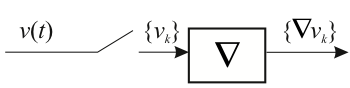
\includegraphics{pictures/cse1.png}}
  \end{center}
  \item This can be represented in transform as
  \begin{center}
    \resizebox{180pt}{!}{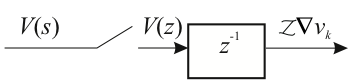
\includegraphics{pictures/cse2.png}}
  \end{center}
\end{itemize}
\end{slide}

\begin{slide}\label{slide:l11s2}
  \heading{Sampling a Delayed Signal}
\begin{itemize}
  \item The same result could be obtained by delaying the continuous
    signal and then sampling.
  \begin{center}
  \resizebox{180pt}{!}{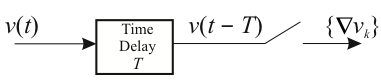
\includegraphics{pictures/cse3.png}}
  \end{center}
  \item Which can be represented in transform as
  \begin{center}
   \resizebox{180pt}{!}{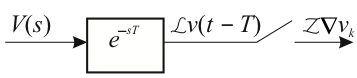
\includegraphics{pictures/cse4.png}}
  \end{center}
\end{itemize}
\end{slide}

From the preceding arguments
  \begin{equation}
    \label{eq:l11e1}
    z^{-1} = e^{-sT}
  \end{equation}
  That is 
  \begin{equation}
    \label{eq:l11e2}
    z=e^{sT}
  \end{equation}
or 
\begin{equation}
  \label{eq:l11e3}
  s=\frac{1}{T}\ln z
\end{equation}
This is the fundamental relationship of equivalence. Before using it,
we must see how a continuous signal is reconstructed from a digital
signal. This is accomplished by means of a ``\emph{Digital-to-Analogue
Converter}''

\section*{Digital-to-Analogue
Converter}
The simplest converter is a ``\emph{Zero-Order Hold}'' (see
Fig.~\ref{fig:l11f1}). This acts the opposite way to a sampler.
\begin{figure}[htbp]
  \begin{center}
    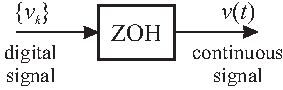
\includegraphics{pictures/zoh.pdf}
    \caption{Zero-Order Hold}
    \label{fig:l11f1}
  \end{center}
\end{figure}

During each sample period, the device holds the output $v(t)$ constant
at the current value of the digital signal $v_k$. That is
\begin{equation}
  \label{eq:l11e4}
  v(t) = v_k\ \mathrm{for}\ kT \le t < (k+1)T
\end{equation}
This generates a stepwise continuous signal $v(t)$ which at the
sampling instants is equal to the continuous signal from which the
digital signal ${v_k}$ was generated (\sref{slide:l11s3}).

\begin{slide}\label{slide:l11s3}
  \heading{Step-wise continuous signal}
  This represents the output of the zero-order hold $v(t) = v_k$ for
  $kT \le t < (k+1)T$.\\
  \begin{center}
\resizebox{300pt}{!}{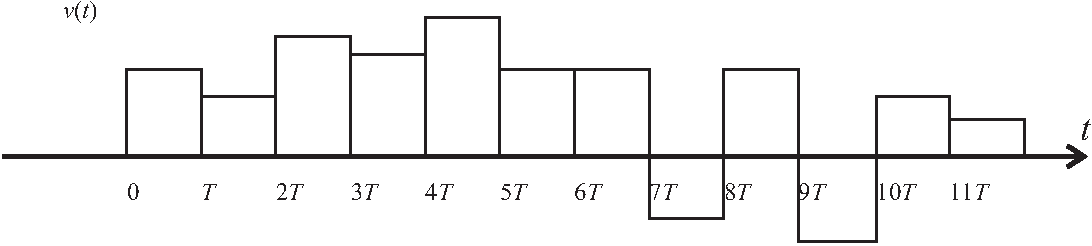
\includegraphics{pictures/steps.pdf}}
  \end{center}
\end{slide}

The signal may be considered as an infinite number of pulses of which
  the $k$-th is that shown in \sref{slide:l11s4}. To model such a
  signal we use the so-called ``\emph{gating}'' property of the
  time-delayed unit-step function $\epsilon(t)$ illustrated in \sref{slide:l11s5}.

\begin{slide}\label{slide:l11s4}
  \heading{The $k$-th ``Pulse''}

  \begin{center}
\resizebox{300pt}{!}{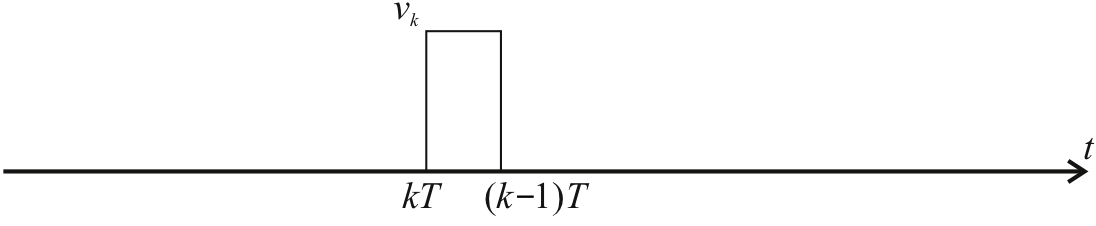
\includegraphics{pictures/pulse.png}}
  \end{center}
\end{slide}

\begin{slide}\label{slide:l11s5}
  \heading{The Gating Function}
  \begin{center}
\resizebox{300pt}{!}{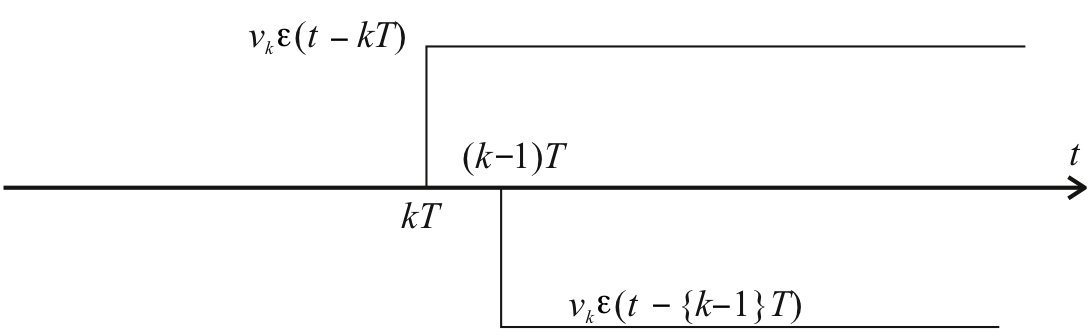
\includegraphics{pictures/gate.png}}
  \end{center}
\end{slide}

The opening ``gate'' is given by $v_k \epsilon (t-kT)$, a step of height
$v_k$, which is activated at $t=kT$ seconds. The gate is ``closed'' by
a negative going unit step, also of height $v_k$, which is activated
at $t=\{k+1\}T$ seconds. The sum of these two signals is 
\begin{eqnarray*}
  p(t) &=& v_k \epsilon(t - kT) - v_k \epsilon(t - \{k+1\}T)\\
       &=& v_k\left[\epsilon(t - kT) - v_k \epsilon(t - \{k+1\}T)\right]
\end{eqnarray*}
So for the sequence:
\begin{equation}
  \label{eq:l11e5}
  v(t) = \sum_{k=0}^{\infty} v_k\left[\epsilon(t - kT) - v_k \epsilon(t - \{k+1\}T)\right]
\end{equation}
In transform form this is
\begin{eqnarray*}
  V(s) &=& \sum_{k=0}^{\infty} v_k\left(\frac{1}{s}e^{-kTs} -
  \frac{1}{s}e^{-\left\{k+1\right\}Ts}\right)\\
       &=& \frac{1}{s}\left(1-e^{-Ts}\right) \sum_{k=0}^{\infty} v_k
  e^{-kTs}\\
       &=& \frac{1}{s}\left(1-z^{-1}\right) \sum_{k=0}^{\infty} v_k
  z^{-k}\\
       &=& \frac{1}{s}\,\frac{z-1}{z}\,V(z)
\end{eqnarray*}

So the zero-order hold is represented by the mixed transfer function 
\begin{equation}
  \label{eq:l11e10}
  G_{\mathrm{zoh}}=\frac{1}{s}\,\frac{z-1}{z}
\end{equation}
as shown in Fig.~\ref{fig:l11f2}.
\begin{figure}[htbp]
  \begin{center}
    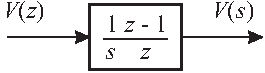
\includegraphics{pictures/zohtf.pdf}
    \caption{Transfer Function of the Zero-Order Hold}
    \label{fig:l11f2}
  \end{center}
\end{figure}

We can now design a `hold-equivalent' digital system as shown in
\sref{slide:l11s10}. From the diagram
\begin{eqnarray*}
  Y(z) &=& H(z) U(z)\\
  Y(z) &=& \mathcal{Z} Y(s)\\
       &=& \mathcal{Z} \frac{1}{s} H(s) \frac{z-1}{z} U(z)
\end{eqnarray*}
so
\begin{eqnarray}\label{eq:l11e14}
  H(z) &=& \frac{z-1}{z} \mathcal{Z} \frac{H(s)}{s}
\end{eqnarray}

\begin{slide}\label{slide:l11s10}
  \heading{Hold-Equivalent Digital System}
  \resizebox{300pt}{!}{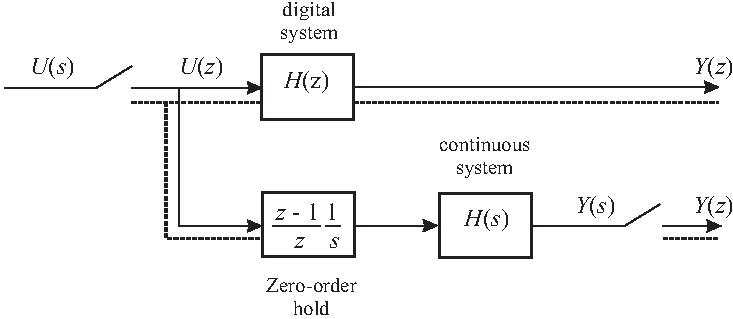
\includegraphics{pictures/holdequiv.pdf}}
\end{slide}

\begin{slide}\label{slide:l11s11}
  \heading{Example}
  If \[H(s) = \frac{a}{s+a}\] then
  \begin{eqnarray*}
    H(z) &=& \frac{z-1}{z}\mathcal{Z} \frac{a}{s(s+a)}\\
         &=& \frac{z-1}{z} \frac{z(1-e^{-aT})}{(z-1)(z-e^{-aT})}\\
         &=& \frac{1-e^{aT}}{z-e^{-aT}}.
  \end{eqnarray*}
\end{slide}

\section*{Other Continuous System Equivalences}

An alternative approach is to use the relationship \[ s  = \frac{1}{T}
\ln z. \] This cannot be substituted into a transfer function directly
as the result is not rational, but an approximation may be used. 

Three approximations, obtained from numerical integration, may be
used. These are illustrated in \sref{slide:l11s20} to \sref{slide:l11s22}

\begin{slide}\label{slide:l11s20}
  \heading{Forward Rectangular Approximation}
  
  \begin{eqnarray*}
     s &=& \frac{z-1}{T} \\
     z &=& 1 + sT
  \end{eqnarray*}
  compare with $$z = e^{sT} = 1 + sT + 1/2 s^2T^2 + 1/6 s^3T^3 + \cdots$$
\end{slide}

\begin{slide}\label{slide:l11s21}
  \heading{Backward Rectangular Approximation}
  
  \begin{eqnarray*}
     s &=& \frac{z-1}{Tz} \\
     z &=& \frac{1}{1 + sT}
  \end{eqnarray*}
  compare expansion $$z=(1-sT)^{-1} = 1 + sT + s^2T^2 + s^3T^3
 + \cdots$$  with $$z = e^{sT} = 1 + sT + 1/2 s^2T^2 + 1/6 s^3T^3 + \cdots$$
\end{slide}

\begin{slide}\label{slide:l11s22}
  \heading{Trapezoidal Approximation}
  
  \begin{eqnarray*}
     s &=& \frac{2}{T}\, \frac{z-1}{z+1} \\
     z &=& \frac{1 + 1/2 sT}{1 - 1/2 sT}
  \end{eqnarray*}
  compare expansion $$z=(1+ 1/2 sT)(1- 1/2 sT)^{-1} = 1 + sT + 1/2
 s^2T^2 + 1/4 s^3T^3
 + \cdots$$  with $$z = e^{sT} = 1 + sT + 1/2 s^2T^2 + 1/6 s^3T^3 + \cdots$$
\end{slide}

The approximation shown in the last slide (\sref{slide:l11s22}) is
best, and is known as ``\emph{Tustin's Bilinear Transformation}''.

\begin{slide}\label{slide:l11s23}
  \heading{Example}
  If \[H(s) = \frac{a}{s+a}\] then the bilinear transformation gives a
  digital system with transfer function
  \begin{eqnarray*}
    H(z)&=& \frac{a}{\frac{2}{T}\,\frac{z-1}{z+1}+a} \\
        &=& \frac{\left(\frac{aT/2}{1+aT/2}\right)(z+1)}{z-\left(\frac{1-aT/2}{1+aT/2}\right)}.
  \end{eqnarray*}
\end{slide}

%----------------------------------------------------------------
% The end of notes
% ----------------------------------------------------------------
\endinput

% Local Variables:
% TeX-master: "lecture03"
% End:
